\documentclass[tikz,border=5pt]{standalone}
\usepackage{amssymb,amsmath, mathtools}
\newcommand{\C}{\mathbb{C}}
\newcommand{\CP}{\mathbb{CP}}
\begin{document}
%========================================================
% FIGURE 1: X = CP^1 (Riemann sphere)
%========================================================
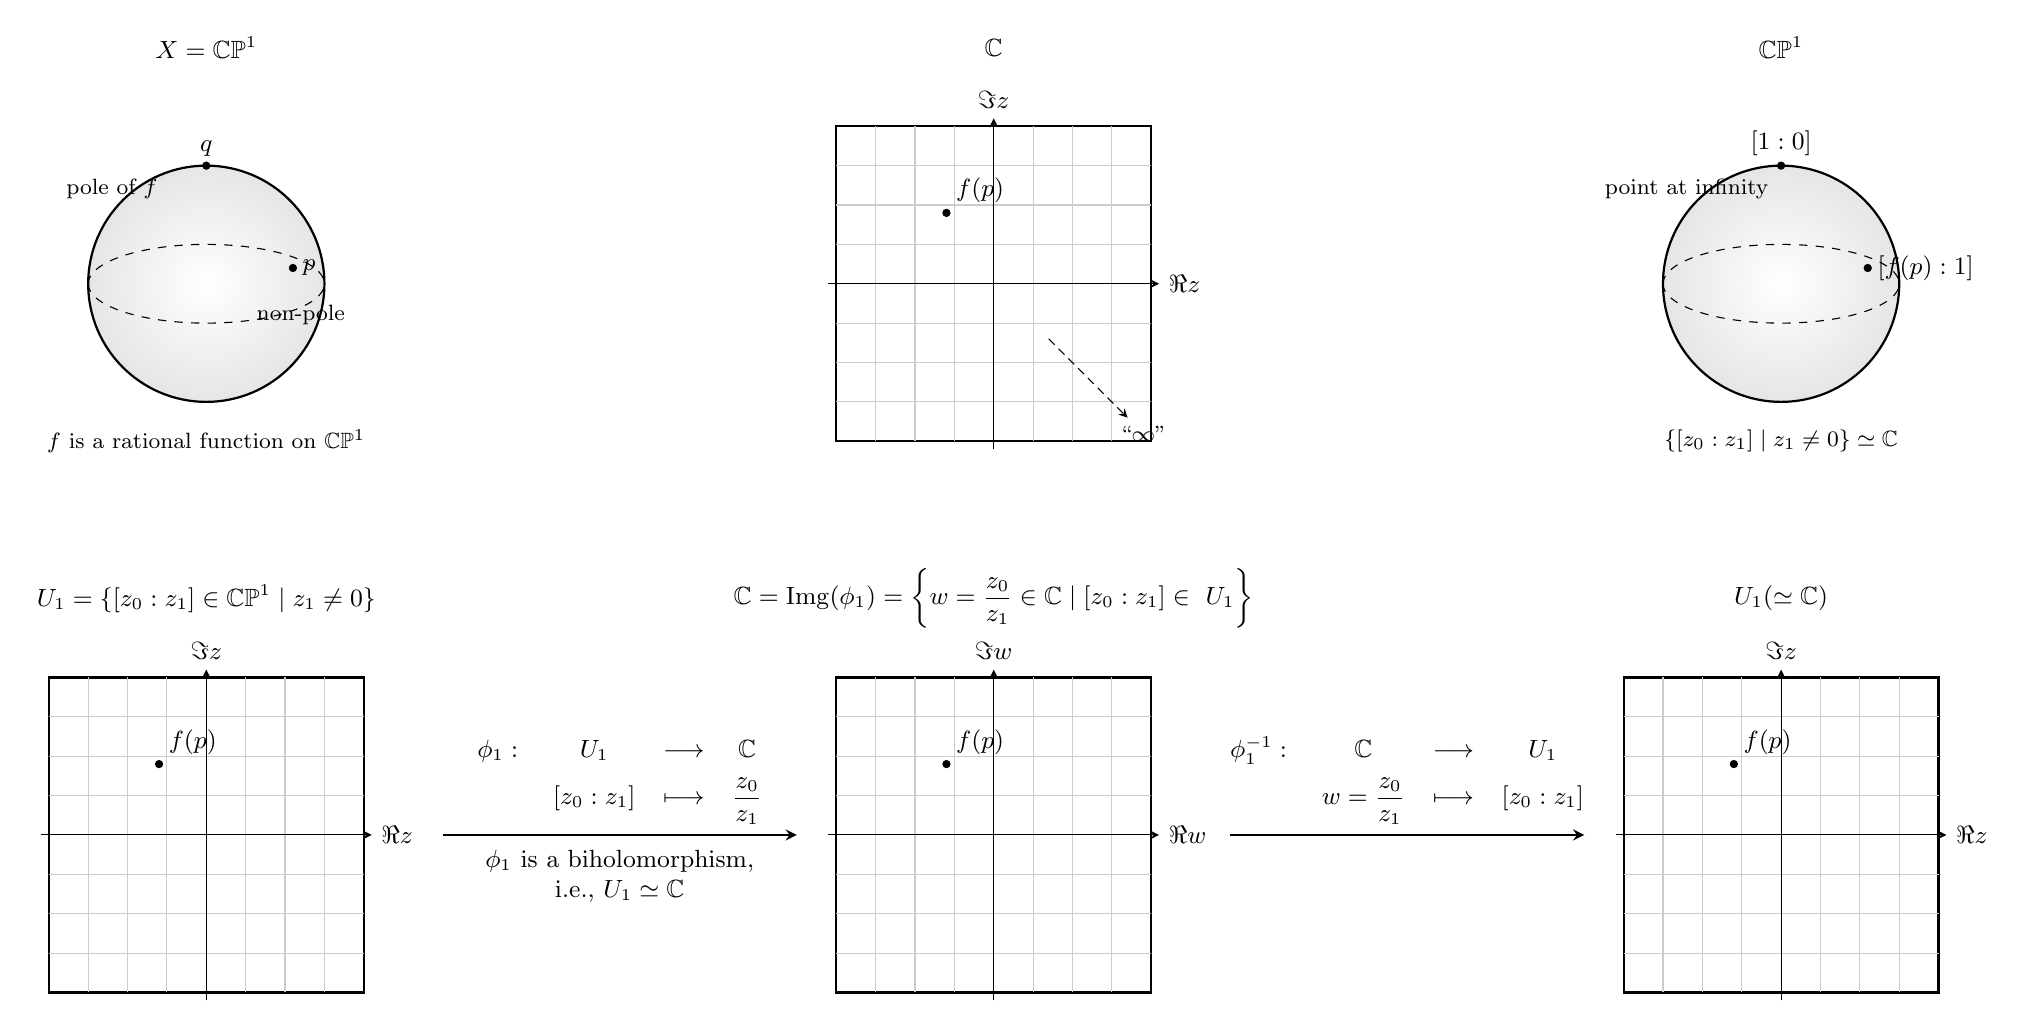
\begin{tikzpicture}[font=\small,>=stealth]

%----------------------------
% Left: Domain X = CP^1
%----------------------------
\begin{scope}[shift={(-10,0)}]
	% Sphere for X
	\shade[inner color=white, outer color=gray!20, draw=black, thick]
	(0,0) circle (1.5);
	\node at (0,3) {$X=\mathbb{CP}^1$};
	
	% north pole (could be a pole of f)
	\fill (0,1.5) circle (1.5pt);
	\node[above] at (0,1.5) {$q$};
	\node at (-1.2,1.2) {\footnotesize pole of $f$};
	
	% equator point p (non-pole)
	\fill (1.1,0.2) circle (1.5pt);
	\node[right] at (1.1,0.2) {$p$};
	\node at (1.2,-0.4) {\footnotesize non-pole};
	% Equator: affine chart U_1
	\draw[dashed] (-1.5,0) arc (180:360:1.5 and 0.5);
	\draw[dashed] (-1.5,0) arc (180:0:1.5 and 0.5);
	% optional label: f meromorphic on CP^1 = rational function
	\node at (0,-2.0) {\footnotesize $f$ is a rational function on $\mathbb{CP}^1$};
\end{scope}

%----------------------------
% Middle: Complex plane C
%----------------------------
\begin{scope}
	% Draw a square region for C
	\draw[thick] (-2,-2) rectangle (2,2);
	\node at (0,3) {$\mathbb{C}$};
	
	% Light grid inside
	\foreach \x in {-1.5,-1,...,1.5}
	\draw[gray!40] (\x,-2) -- (\x,2);
	\foreach \y in {-1.5,-1,...,1.5}
	\draw[gray!40] (-2,\y) -- (2,\y);
	
	% Axes
	\draw[->] (-2.1,0) -- (2.1,0) node[right] {\(\Re z\)};
	\draw[->] (0,-2.1) -- (0,2.1) node[above] {\(\Im z\)};
	
	% image of p under f
	\fill (-0.6,0.9) circle (1.5pt) node[above right] {\(f(p)\)};
	
	% suggest f(q) "goes to infinity" (pole)
	\draw[->,densely dashed] (0.7,-0.7) -- (1.7,-1.7);
	\node at (1.9,-1.9) {\footnotesize ``$\infty$''};
\end{scope}

%----------------------------
% Right: Target CP^1
%----------------------------
\begin{scope}[shift={(10,0)}]
	% Sphere for CP^1
	\shade[inner color=white, outer color=gray!20, draw=black, thick]
	(0,0) circle (1.5);
	\node at (0,3) {$\mathbb{CP}^1$};
	
	% north pole = [1:0]
	\fill (0,1.5) circle (1.5pt);
	\node[above] at (0,1.5) {$[1\;\text{:}\;0]$};
	\node at (-1.2,1.2) {\footnotesize point at infinity};
	
	% equator point = [f(p):1]
	\fill (1.1,0.2) circle (1.5pt);
	\node[right] at (1.1,0.2) {$[f(p)\;\text{:}\;1]$};
	
	% Equator: affine chart U_1
	\draw[dashed] (-1.5,0) arc (180:360:1.5 and 0.5);
	\draw[dashed] (-1.5,0) arc (180:0:1.5 and 0.5);
	
	% note affine chart below
	\node at (0,-2.0) {\footnotesize $\{[z_0\;\text{:}\;z_1]\mid z_1\neq 0\}\simeq\C$};
\end{scope}

%%----------------------------
%% Arrows: f, F, inclusion i
%%----------------------------
%
%% arrow f: X -> C (from p)
%\draw[->,thick]
%(-3.7,0.2) .. controls (-2,1.4) .. (-1.0,0.9)
%node[midway,above] {$f$};
%
%% arrow F: X -> CP^1 (from p)
%\draw[->,thick]
%(-3.7,0.2) .. controls (0,2.6) .. (3.7,0.2)
%node[midway,above] {$F$};
%
%% image of pole q under F: q -> [1:0]
%\draw[->,thick]
%(-3.5,1.5) .. controls (0,3.0) .. (4.2,1.6);
%\node at (0,3.1) {\footnotesize $q\mapsto[1:0]$};
%
%% inclusion i: C -> CP^1, z |-> [z:1]
%\draw[->,thick]
%(2.1,-0.1) .. controls (3.0,-0.8) .. (4.1,-0.8)
%node[midway,below] {$i$};
%\node at (3.1,-1.5) {\footnotesize $i(z)=[z:1]$};



\begin{scope}[shift={(-10,-7)}]
	% Draw a square region for C
	\draw[thick] (-2,-2) rectangle (2,2);
	\node[align=center] at (0,3) {$U_1=\{[z_0:z_1]\in\CP^1\mid z_1\neq 0\}$};
	% Light grid inside
	\foreach \x in {-1.5,-1,...,1.5}
	\draw[gray!40] (\x,-2) -- (\x,2);
	\foreach \y in {-1.5,-1,...,1.5}
	\draw[gray!40] (-2,\y) -- (2,\y);
	% Axes
	\draw[->] (-2.1,0) -- (2.1,0) node[right] {\(\Re z\)};
	\draw[->] (0,-2.1) -- (0,2.1) node[above] {\(\Im z\)};
	% image of p under f
	\fill (-0.6,0.9) circle (1.5pt) node[above right] {\(f(p)\)};
\end{scope}
\draw[->,thick] (-7,-7) -- (-2.5,-7)
node[midway,above] {$\begin{array}{cccc}
		\phi_1\;\text{:}\; & U_1 & \longrightarrow & \C \\ [4pt]
		& [z_0:z_1] & \longmapsto & \displaystyle\frac{z_0}{z_1}
	\end{array}$};
\node[below=2, align=center] at (-4.75, -7) {$\phi_1$ is a biholomorphism,\\ i.e., $U_1\simeq\C$};
\begin{scope}[shift={(0,-7)}]
	% Draw a square region for C
	\draw[thick] (-2,-2) rectangle (2,2);
	\node[align=center] at (0,3) {$\mathbb{C}=\mathrm{Img}(\phi_1)=\left\{\displaystyle w=\frac{z_0}{z_1}\in\C\mid[z_0:z_1]\in\ U_1\right\}$};
	
	% Light grid inside
	\foreach \x in {-1.5,-1,...,1.5}
	\draw[gray!40] (\x,-2) -- (\x,2);
	\foreach \y in {-1.5,-1,...,1.5}
	\draw[gray!40] (-2,\y) -- (2,\y);
	
	% Axes
	\draw[->] (-2.1,0) -- (2.1,0) node[right] {\(\Re w\)};
	\draw[->] (0,-2.1) -- (0,2.1) node[above] {\(\Im w\)};
	
	% image of p under f
	\fill (-0.6,0.9) circle (1.5pt) node[above right] {\(f(p)\)};
%	% suggest f(q) "goes to infinity" (pole)
%	\draw[->,densely dashed] (0.7,-0.7) -- (1.7,-1.7);
%	\node at (1.9,-1.9) {\footnotesize ``$\infty$''};
\end{scope}
\draw[->,thick] (3,-7) -- (7.5,-7)
node[midway,above] {$\begin{array}{cccc}
		\phi_1^{-1}\;\text{:}\; & \C & \longrightarrow & U_1 \\ [4pt]
		& w=\displaystyle\frac{z_0}{z_1} & \longmapsto & [z_0:z_1]
	\end{array}$};
\begin{scope}[shift={(10,-7)}]
	% Draw a square region for C
	\draw[thick] (-2,-2) rectangle (2,2);
	\node at (0,3) {$U_1(\simeq\C)$};
	
	% Light grid inside
	\foreach \x in {-1.5,-1,...,1.5}
	\draw[gray!40] (\x,-2) -- (\x,2);
	\foreach \y in {-1.5,-1,...,1.5}
	\draw[gray!40] (-2,\y) -- (2,\y);
	
	% Axes
	\draw[->] (-2.1,0) -- (2.1,0) node[right] {\(\Re z\)};
	\draw[->] (0,-2.1) -- (0,2.1) node[above] {\(\Im z\)};
	
	% image of p under f
	\fill (-0.6,0.9) circle (1.5pt) node[above right] {\(f(p)\)};
%	% suggest f(q) "goes to infinity" (pole)
%	\draw[->,densely dashed] (0.7,-0.7) -- (1.7,-1.7);
%	\node at (1.9,-1.9) {\footnotesize ``$\infty$''};
\end{scope}
\end{tikzpicture}	
\end{document}